%!TEX root = ../main.tex
\section{Testing}

The software development method used to implement setlx2py was chosen to be test-driven development (\gls{tdd}). The biggest reason for that was the fact that small changes in the parser might result in hard-to-find errors. In addition to that, the code generation has influence of many features which the SetlX language offers. A small change can render many of them wrong, and tests are used to catch them.

It proved to reduce the amount of debugging, and assures a high quality from start to end. Also, refactoring or extensions in the future (especially by new authors) which break the functionallity are detected very early. Last but not least, the tests serve as documentation of the language.

\subsection{Test-driven development}

There are many definitions of test driven development, one of the most popular is the following by Robert Cecil Martin, a leader of the Agile and Clean Code Movement. It can be found in \cite{tdd} and reads the following:

\begin{enumerate}
\item You are not allowed to write any production code unless it is to make a failing unit test pass.
\item You are not allowed to write any more of a unit test than is sufficient to fail; and compilation failures are failures.
\item You are not allowed to write any more production code than is sufficient to pass the one failing unit test.
\end{enumerate}

Therefore, each token of the lexer, each grammar rule, each code generation, all builtins have corresponding tests, etc \ldots which were written before actual fucntionality was implemented for them. Setlx2py has more lines of tests than implementation code.

It may be the case that different methodology would achieve the same result, but TDD worked well in this project.

\clearpage
\subsection{Running the tests}

The tests are implemented using the nosetest framework for Python. They can be run with

\begin{lstlisting}{language=bash}
# nosetests 
\end{lstlisting}

on Linux/Mac or 

\begin{lstlisting}{language=bash}
# nosetests.exe
\end{lstlisting}

on Windows while being in the setlx2py root directory.

\begin{figure}[htb]
	\centering
	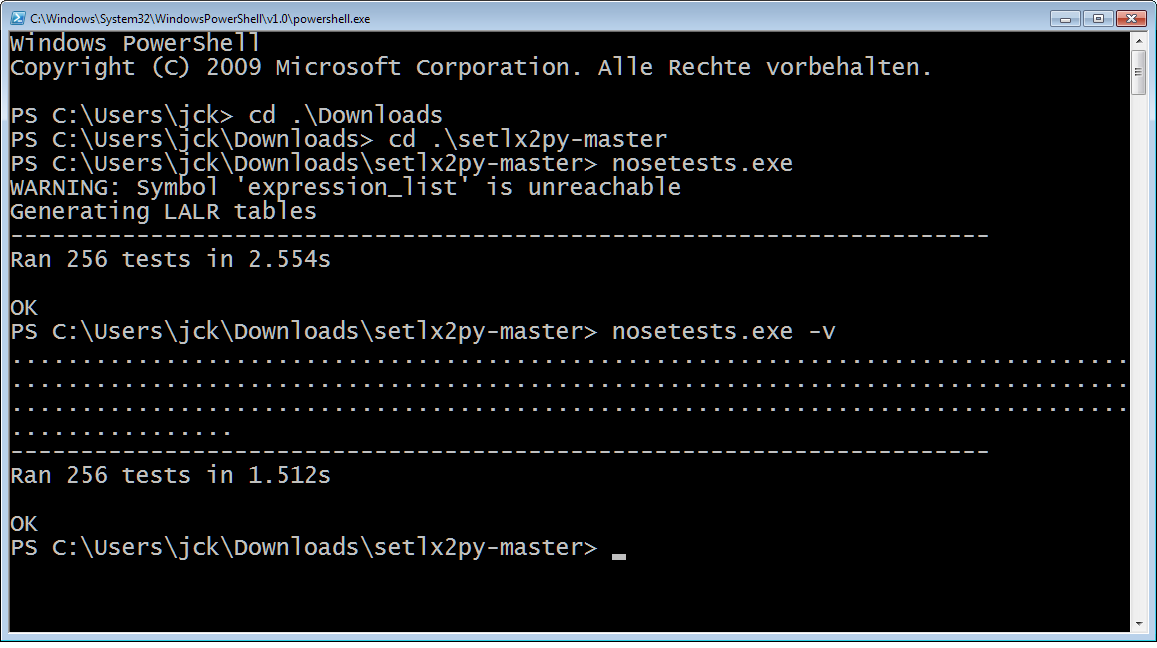
\includegraphics[width=0.8\textwidth]{img/run-nose.png}
	\caption{Output of nosetest: All tests passed}

\end{figure}